
\begin{frame}
    \frametitle{Exercise 3.4 - 16}
    \textit{Problem Statement}\\
    Give an example of a topological space which is Hausdorff but not
    metrizable.
\end{frame}

\begin{frame}
    \frametitle{Examining the problem}

    We just proved Metrizable \(\Leftrightarrow\) Hausdorff, so what gives?
    \pause
    There is something quite important we used to establish all the ideas in
    that problem. \pause \emph{Finiteness.}

\end{frame}

\begin{frame}
    \frametitle{Morphing Relationships}
    \centering
    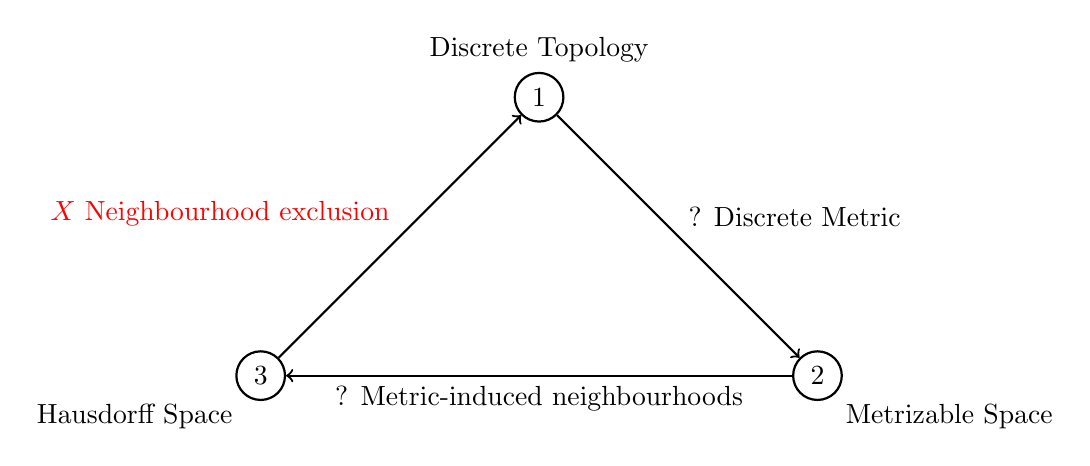
\begin{tikzpicture}[node distance={5cm}, thick, main/.style = {draw, circle}]
        \node[main, label=above:Discrete Topology] (1)                      {\(1\)};
        \node[main, label=below right:Metrizable Space] (2) [below right of=1]    {\(2\)};
        \node[main, label=below left:Hausdorff Space] (3) [below left of=1]      {\(3\)};

        % \pause

        \draw[->] (1) -- node[midway, above right] {? Discrete Metric} (2);
        \draw[->] (2) -- node[midway, below] {? Metric-induced neighbourhoods} (3);
        \draw[->] (3) -- node[midway, above left] {\textcolor{red}{\(X\) Neighbourhood exclusion}} (1);

    \end{tikzpicture}

\end{frame}

\begin{frame}
    \frametitle{Chasing Broken Bridges}

    We are now looking for a Hausdorff space that is not metrizable. It cannot
    be discrete, since we have the discrete metric for it, regardless of
    finiteness, i.e., the implication edge \(1\rightarrow 2\) holds without
    finiteness too.

\end{frame}

\begin{frame}
    \frametitle{Morphing Relationships}
    \centering
    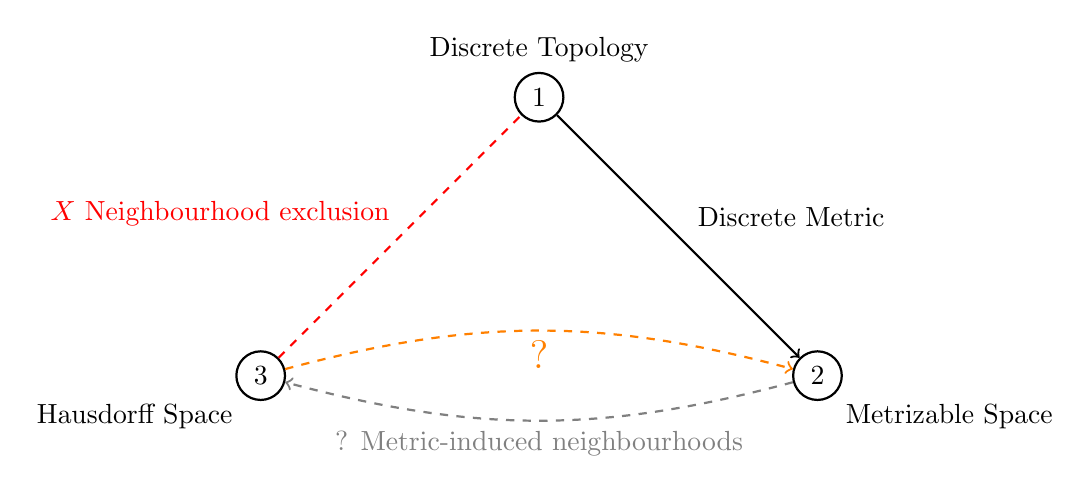
\begin{tikzpicture}[node distance={5cm}, thick, main/.style = {draw, circle}]
        \node[main, label=above:Discrete Topology] (1)                      {\(1\)};
        \node[main, label=below right:Metrizable Space] (2) [below right of=1]    {\(2\)};
        \node[main, label=below left:Hausdorff Space] (3) [below left of=1]      {\(3\)};

        % \pause

        \draw[->] (1) -- node[midway, above right] {\(\checkmark\) Discrete Metric} (2);
        \draw[->, color=orange] (3) [bend right=-15] to node[midway, below] {\Large ?} (2) [dashed];
        \draw[->, color=gray] (2) [bend left=15] to node[midway, below] {? Metric-induced neighbourhoods} (3) [dashed];
        \draw[color=red] (3) -- node[midway, above left] {\textcolor{red}{\(X\) Neighbourhood exclusion}}(1) [dashed];

    \end{tikzpicture}

    \pause

    We have lost some information about the internal relationships while
    breaking one edge. \pause If finiteness doesn't break things enough,
    what did we use that might?
    % So our diagram order was chosen carefully to be annoying

\end{frame}

% \begin{frame}
%     \frametitle{Countability}

%     We broke our `weakest link' by removing the assumption of being able to
%     finitely count the set.\pause The next step is to remove the assumption that
%     we are able to \emph{count at all}.
%     % The discreteness was a ruse all along

% \end{frame}

\begin{frame}
    \frametitle{A Chasm}

    We construct a topology from a metric space by constructing open balls
    around points. \pause So, perhaps we can break metrizability by taking a
    Hausdorff space, and creating gaps in it that cannot be worked around with a
    metric. % real numbers are in particular, always finite individually

\end{frame}

\begin{frame}

    Combining everything, consider the space \((\reals, \tau)\) with \(\tau\)
    being the usual topology on the real line. It is clearly Hausdorff, and
    metrizable. \pause Construct from this a new space \(*\reals\) from \reals\,
    with an added point \(\omega\), a number larger than any finite real. Choose
    the set \(\{\omega\}\) to additionally be open. \pause We see that there are
    suddenly issues with defining a metric on this space.

\end{frame}

\begin{frame}

    Suppose we were able to metrize this space. That would imply we have defined
    a \emph{real} distance between all points on the real line and \(\omega\)
    \pause, but this would imply that \(\omega\) is contained within some finite
    open balls centered at said points. Intuitively, this does not make any
    sense per the definition of \(\omega\).

\end{frame}

\begin{frame}

    \begin{proof}[Non-metrizability of \(*\reals\)]
        If possible, suppose there exists a metric such that it induces the
        defined topology on \(*\reals\), \(d:*\reals \times *\reals \to
        \reals\), defined as usual over the `finite' numbers. \pause So
        \(\exists f:\reals \to \reals, \text{such that }\forall x \in \reals
        \;d(x, \omega) = f(x)\). Now, pick any two points \(x, y \not =
        \omega\), such that \(d(x, y) = a\) for some real \(a\). 
        
        \pause 
        Then by the triangle inequality, we must have
        \begin{gather*}
            d(x, y) \leq d(x, \omega) + d(\omega, y) \textnormal{ , so} \\
            a \leq f(x) + f(y)~.
        \end{gather*}

        Since \(a, x, \textnormal{and } y\) were arbitrary, \(f(x)\) must be
        unbounded \(\forall x\), and thus \(d\) is not a proper metric. This
        happens because \(\omega\) is a transfinite number. We have a
        contradiction. 
    \end{proof}

\end{frame}